\documentclass[twoside]{book}

% Packages required by doxygen
\usepackage{calc}
\usepackage{doxygen}
\usepackage{graphicx}
\usepackage[utf8]{inputenc}
\usepackage{makeidx}
\usepackage{multicol}
\usepackage{multirow}
\usepackage{textcomp}
\usepackage[table]{xcolor}

% NLS support packages
\usepackage[french]{babel}

% Font selection
\usepackage[T1]{fontenc}
\usepackage{mathptmx}
\usepackage[scaled=.90]{helvet}
\usepackage{courier}
\usepackage{amssymb}
\usepackage{sectsty}
\renewcommand{\familydefault}{\sfdefault}
\allsectionsfont{%
  \fontseries{bc}\selectfont%
  \color{darkgray}%
}
\renewcommand{\DoxyLabelFont}{%
  \fontseries{bc}\selectfont%
  \color{darkgray}%
}

% Page & text layout
\usepackage{geometry}
\geometry{%
  a4paper,%
  top=2.5cm,%
  bottom=2.5cm,%
  left=2.5cm,%
  right=2.5cm%
}
\tolerance=750
\hfuzz=15pt
\hbadness=750
\setlength{\emergencystretch}{15pt}
\setlength{\parindent}{0cm}
\setlength{\parskip}{0.2cm}
\makeatletter
\renewcommand{\paragraph}{%
  \@startsection{paragraph}{4}{0ex}{-1.0ex}{1.0ex}{%
    \normalfont\normalsize\bfseries\SS@parafont%
  }%
}
\renewcommand{\subparagraph}{%
  \@startsection{subparagraph}{5}{0ex}{-1.0ex}{1.0ex}{%
    \normalfont\normalsize\bfseries\SS@subparafont%
  }%
}
\makeatother

% Headers & footers
\usepackage{fancyhdr}
\pagestyle{fancyplain}
\fancyhead[LE]{\fancyplain{}{\bfseries\thepage}}
\fancyhead[CE]{\fancyplain{}{}}
\fancyhead[RE]{\fancyplain{}{\bfseries\leftmark}}
\fancyhead[LO]{\fancyplain{}{\bfseries\rightmark}}
\fancyhead[CO]{\fancyplain{}{}}
\fancyhead[RO]{\fancyplain{}{\bfseries\thepage}}
\fancyfoot[LE]{\fancyplain{}{}}
\fancyfoot[CE]{\fancyplain{}{}}
\fancyfoot[RE]{\fancyplain{}{\bfseries\scriptsize Généré le Mardi 15 Avril 2014 09\-:22\-:34 pour D\-G\-L par Doxygen }}
\fancyfoot[LO]{\fancyplain{}{\bfseries\scriptsize Généré le Mardi 15 Avril 2014 09\-:22\-:34 pour D\-G\-L par Doxygen }}
\fancyfoot[CO]{\fancyplain{}{}}
\fancyfoot[RO]{\fancyplain{}{}}
\renewcommand{\footrulewidth}{0.4pt}
\renewcommand{\chaptermark}[1]{%
  \markboth{#1}{}%
}
\renewcommand{\sectionmark}[1]{%
  \markright{\thesection\ #1}%
}

% Indices & bibliography
\usepackage{natbib}
\usepackage[titles]{tocloft}
\setcounter{tocdepth}{3}
\setcounter{secnumdepth}{5}
\makeindex

% Hyperlinks (required, but should be loaded last)
\usepackage{ifpdf}
\ifpdf
  \usepackage[pdftex,pagebackref=true]{hyperref}
\else
  \usepackage[ps2pdf,pagebackref=true]{hyperref}
\fi
\hypersetup{%
  colorlinks=true,%
  linkcolor=blue,%
  citecolor=blue,%
  unicode%
}

% Custom commands
\newcommand{\clearemptydoublepage}{%
  \newpage{\pagestyle{empty}\cleardoublepage}%
}


%===== C O N T E N T S =====

\begin{document}

% Titlepage & ToC
\hypersetup{pageanchor=false}
\pagenumbering{roman}
\begin{titlepage}
\vspace*{7cm}
\begin{center}%
{\Large D\-G\-L \\[1ex]\large 20140414 }\\
\vspace*{1cm}
{\large Généré par Doxygen 1.8.6}\\
\vspace*{0.5cm}
{\small Mardi 15 Avril 2014 09:22:34}\\
\end{center}
\end{titlepage}
\clearemptydoublepage
\tableofcontents
\clearemptydoublepage
\pagenumbering{arabic}
\hypersetup{pageanchor=true}

%--- Begin generated contents ---
\chapter{Index des espaces de nommage}
\input{namespaces}
\chapter{Index hiérarchique}
\section{Hiérarchie des classes}
Cette liste d'héritage est classée approximativement par ordre alphabétique \-:\begin{DoxyCompactList}
\item \contentsline{section}{C\-G\-L\-Object}{\pageref{d2/d76/class_c_g_l_object}}{}
\begin{DoxyCompactList}
\item \contentsline{section}{C\-G\-L\-Effect}{\pageref{dc/d8a/class_c_g_l_effect}}{}
\begin{DoxyCompactList}
\item \contentsline{section}{C\-G\-L\-Color}{\pageref{d7/dd6/class_c_g_l_color}}{}
\item \contentsline{section}{C\-G\-L\-Position}{\pageref{de/d31/class_c_g_l_position}}{}
\item \contentsline{section}{C\-G\-L\-Rotation}{\pageref{d4/dd5/class_c_g_l_rotation}}{}
\begin{DoxyCompactList}
\item \contentsline{section}{C\-G\-L\-Rotation\-Speed}{\pageref{d4/d9e/class_c_g_l_rotation_speed}}{}
\end{DoxyCompactList}
\item \contentsline{section}{C\-G\-L\-Scale}{\pageref{dd/dd7/class_c_g_l_scale}}{}
\end{DoxyCompactList}
\item \contentsline{section}{C\-G\-L\-Item}{\pageref{d7/d2f/class_c_g_l_item}}{}
\begin{DoxyCompactList}
\item \contentsline{section}{C\-G\-L\-Boite}{\pageref{dd/daf/class_c_g_l_boite}}{}
\item \contentsline{section}{C\-G\-L\-Circle}{\pageref{d3/d05/class_c_g_l_circle}}{}
\item \contentsline{section}{C\-G\-L\-Dot}{\pageref{da/d38/class_c_g_l_dot}}{}
\item \contentsline{section}{C\-G\-L\-Line}{\pageref{d9/dfe/class_c_g_l_line}}{}
\item \contentsline{section}{C\-G\-L\-Polygon}{\pageref{d1/db6/class_c_g_l_polygon}}{}
\item \contentsline{section}{C\-G\-L\-Quad}{\pageref{df/d41/class_c_g_l_quad}}{}
\item \contentsline{section}{C\-G\-L\-Robot1}{\pageref{d8/dbf/class_c_g_l_robot1}}{}
\item \contentsline{section}{C\-G\-L\-Triangle}{\pageref{d1/d68/class_c_g_l_triangle}}{}
\end{DoxyCompactList}
\item \contentsline{section}{C\-G\-L\-Special}{\pageref{d0/d14/class_c_g_l_special}}{}
\begin{DoxyCompactList}
\item \contentsline{section}{C\-G\-L\-Camera}{\pageref{de/dee/class_c_g_l_camera}}{}
\item \contentsline{section}{C\-G\-L\-Camera\-List}{\pageref{d4/dad/class_c_g_l_camera_list}}{}
\item \contentsline{section}{C\-G\-L\-Light}{\pageref{da/dc8/class_c_g_l_light}}{}
\item \contentsline{section}{C\-G\-L\-Scene}{\pageref{d9/d85/class_c_g_l_scene}}{}
\item \contentsline{section}{C\-G\-L\-Window}{\pageref{dd/d40/class_c_g_l_window}}{}
\item \contentsline{section}{C\-G\-L\-World}{\pageref{db/da4/class_c_g_l_world}}{}
\end{DoxyCompactList}
\end{DoxyCompactList}
\item \contentsline{section}{C\-G\-L\-Vector2\-D}{\pageref{d8/d97/class_c_g_l_vector2_d}}{}
\begin{DoxyCompactList}
\item \contentsline{section}{C\-G\-L\-Vector3\-D}{\pageref{d6/df9/class_c_g_l_vector3_d}}{}
\begin{DoxyCompactList}
\item \contentsline{section}{C\-G\-L\-Position}{\pageref{de/d31/class_c_g_l_position}}{}
\item \contentsline{section}{C\-G\-L\-Rotation}{\pageref{d4/dd5/class_c_g_l_rotation}}{}
\item \contentsline{section}{C\-G\-L\-Scale}{\pageref{dd/dd7/class_c_g_l_scale}}{}
\item \contentsline{section}{C\-G\-L\-Vector4\-D}{\pageref{db/d79/class_c_g_l_vector4_d}}{}
\begin{DoxyCompactList}
\item \contentsline{section}{C\-G\-L\-Color}{\pageref{d7/dd6/class_c_g_l_color}}{}
\end{DoxyCompactList}
\end{DoxyCompactList}
\end{DoxyCompactList}
\end{DoxyCompactList}

\chapter{Index des classes}
\section{Liste des classes}
Liste des classes, structures, unions et interfaces avec une brève description \-:\begin{DoxyCompactList}
\item\contentsline{section}{\hyperlink{class_c_g_l_boite}{C\-G\-L\-Boite} }{\pageref{dd/daf/class_c_g_l_boite}}{}
\item\contentsline{section}{\hyperlink{class_c_g_l_camera}{C\-G\-L\-Camera} }{\pageref{de/dee/class_c_g_l_camera}}{}
\item\contentsline{section}{\hyperlink{class_c_g_l_camera_list}{C\-G\-L\-Camera\-List} }{\pageref{d4/dad/class_c_g_l_camera_list}}{}
\item\contentsline{section}{\hyperlink{class_c_g_l_color}{C\-G\-L\-Color} }{\pageref{d7/dd6/class_c_g_l_color}}{}
\item\contentsline{section}{\hyperlink{class_c_g_l_dot}{C\-G\-L\-Dot} }{\pageref{da/d38/class_c_g_l_dot}}{}
\item\contentsline{section}{\hyperlink{class_c_g_l_effect}{C\-G\-L\-Effect} }{\pageref{dc/d8a/class_c_g_l_effect}}{}
\item\contentsline{section}{\hyperlink{class_c_g_l_item}{C\-G\-L\-Item} }{\pageref{d7/d2f/class_c_g_l_item}}{}
\item\contentsline{section}{\hyperlink{class_c_g_l_light}{C\-G\-L\-Light} }{\pageref{da/dc8/class_c_g_l_light}}{}
\item\contentsline{section}{\hyperlink{class_c_g_l_line}{C\-G\-L\-Line} }{\pageref{d9/dfe/class_c_g_l_line}}{}
\item\contentsline{section}{\hyperlink{class_c_g_l_object}{C\-G\-L\-Object} }{\pageref{d2/d76/class_c_g_l_object}}{}
\item\contentsline{section}{\hyperlink{class_c_g_l_position}{C\-G\-L\-Position} }{\pageref{de/d31/class_c_g_l_position}}{}
\item\contentsline{section}{\hyperlink{class_c_g_l_quad}{C\-G\-L\-Quad} }{\pageref{df/d41/class_c_g_l_quad}}{}
\item\contentsline{section}{\hyperlink{class_c_g_l_robot1}{C\-G\-L\-Robot1} }{\pageref{d8/dbf/class_c_g_l_robot1}}{}
\item\contentsline{section}{\hyperlink{class_c_g_l_rotation}{C\-G\-L\-Rotation} }{\pageref{d4/dd5/class_c_g_l_rotation}}{}
\item\contentsline{section}{\hyperlink{class_c_g_l_scale}{C\-G\-L\-Scale} }{\pageref{dd/dd7/class_c_g_l_scale}}{}
\item\contentsline{section}{\hyperlink{class_c_g_l_scene}{C\-G\-L\-Scene} }{\pageref{d9/d85/class_c_g_l_scene}}{}
\item\contentsline{section}{\hyperlink{class_c_g_l_special}{C\-G\-L\-Special} }{\pageref{d0/d14/class_c_g_l_special}}{}
\item\contentsline{section}{\hyperlink{class_c_g_l_triangle}{C\-G\-L\-Triangle} }{\pageref{d1/d68/class_c_g_l_triangle}}{}
\item\contentsline{section}{\hyperlink{class_c_g_l_vector2_d}{C\-G\-L\-Vector2\-D} }{\pageref{d8/d97/class_c_g_l_vector2_d}}{}
\item\contentsline{section}{\hyperlink{class_c_g_l_vector3_d}{C\-G\-L\-Vector3\-D} }{\pageref{d6/df9/class_c_g_l_vector3_d}}{}
\item\contentsline{section}{\hyperlink{class_c_g_l_vector4_d}{C\-G\-L\-Vector4\-D} }{\pageref{db/d79/class_c_g_l_vector4_d}}{}
\item\contentsline{section}{\hyperlink{class_c_g_l_window}{C\-G\-L\-Window} }{\pageref{dd/d40/class_c_g_l_window}}{}
\item\contentsline{section}{\hyperlink{class_c_g_l_world}{C\-G\-L\-World} }{\pageref{db/da4/class_c_g_l_world}}{}
\end{DoxyCompactList}

\chapter{Index des fichiers}
\section{Liste des fichiers}
Liste de tous les fichiers avec une brève description \-:\begin{DoxyCompactList}
\item\contentsline{section}{/home/dagal/git/\-Damier\-G\-L/\-Damier\-G\-L/src/\hyperlink{_damier_g_l_8cpp}{Damier\-G\-L.\-cpp} }{\pageref{db/dec/_damier_g_l_8cpp}}{}
\item\contentsline{section}{/home/dagal/git/\-Damier\-G\-L/\-Damier\-G\-L/src/\-C\-G\-L/\hyperlink{_c_g_l_boite_8cpp}{C\-G\-L\-Boite.\-cpp} }{\pageref{da/d3e/_c_g_l_boite_8cpp}}{}
\item\contentsline{section}{/home/dagal/git/\-Damier\-G\-L/\-Damier\-G\-L/src/\-C\-G\-L/\hyperlink{_c_g_l_boite_8h}{C\-G\-L\-Boite.\-h} }{\pageref{db/d17/_c_g_l_boite_8h}}{}
\item\contentsline{section}{/home/dagal/git/\-Damier\-G\-L/\-Damier\-G\-L/src/\-C\-G\-L/\hyperlink{_c_g_l_camera_8cpp}{C\-G\-L\-Camera.\-cpp} }{\pageref{dd/d43/_c_g_l_camera_8cpp}}{}
\item\contentsline{section}{/home/dagal/git/\-Damier\-G\-L/\-Damier\-G\-L/src/\-C\-G\-L/\hyperlink{_c_g_l_camera_8h}{C\-G\-L\-Camera.\-h} }{\pageref{df/d5b/_c_g_l_camera_8h}}{}
\item\contentsline{section}{/home/dagal/git/\-Damier\-G\-L/\-Damier\-G\-L/src/\-C\-G\-L/\hyperlink{_c_g_l_camera_list_8cpp}{C\-G\-L\-Camera\-List.\-cpp} }{\pageref{df/d1a/_c_g_l_camera_list_8cpp}}{}
\item\contentsline{section}{/home/dagal/git/\-Damier\-G\-L/\-Damier\-G\-L/src/\-C\-G\-L/\hyperlink{_c_g_l_camera_list_8h}{C\-G\-L\-Camera\-List.\-h} }{\pageref{d5/d86/_c_g_l_camera_list_8h}}{}
\item\contentsline{section}{/home/dagal/git/\-Damier\-G\-L/\-Damier\-G\-L/src/\-C\-G\-L/\hyperlink{_c_g_l_color_8cpp}{C\-G\-L\-Color.\-cpp} }{\pageref{da/d19/_c_g_l_color_8cpp}}{}
\item\contentsline{section}{/home/dagal/git/\-Damier\-G\-L/\-Damier\-G\-L/src/\-C\-G\-L/\hyperlink{_c_g_l_color_8h}{C\-G\-L\-Color.\-h} }{\pageref{da/de7/_c_g_l_color_8h}}{}
\item\contentsline{section}{/home/dagal/git/\-Damier\-G\-L/\-Damier\-G\-L/src/\-C\-G\-L/\hyperlink{_c_g_l_dot_8cpp}{C\-G\-L\-Dot.\-cpp} }{\pageref{d2/d5a/_c_g_l_dot_8cpp}}{}
\item\contentsline{section}{/home/dagal/git/\-Damier\-G\-L/\-Damier\-G\-L/src/\-C\-G\-L/\hyperlink{_c_g_l_dot_8h}{C\-G\-L\-Dot.\-h} }{\pageref{d5/d21/_c_g_l_dot_8h}}{}
\item\contentsline{section}{/home/dagal/git/\-Damier\-G\-L/\-Damier\-G\-L/src/\-C\-G\-L/\hyperlink{_c_g_l_effect_8cpp}{C\-G\-L\-Effect.\-cpp} }{\pageref{d7/da1/_c_g_l_effect_8cpp}}{}
\item\contentsline{section}{/home/dagal/git/\-Damier\-G\-L/\-Damier\-G\-L/src/\-C\-G\-L/\hyperlink{_c_g_l_effect_8h}{C\-G\-L\-Effect.\-h} }{\pageref{d7/d27/_c_g_l_effect_8h}}{}
\item\contentsline{section}{/home/dagal/git/\-Damier\-G\-L/\-Damier\-G\-L/src/\-C\-G\-L/\hyperlink{_c_g_l_item_8cpp}{C\-G\-L\-Item.\-cpp} }{\pageref{da/dcb/_c_g_l_item_8cpp}}{}
\item\contentsline{section}{/home/dagal/git/\-Damier\-G\-L/\-Damier\-G\-L/src/\-C\-G\-L/\hyperlink{_c_g_l_item_8h}{C\-G\-L\-Item.\-h} }{\pageref{d2/d5a/_c_g_l_item_8h}}{}
\item\contentsline{section}{/home/dagal/git/\-Damier\-G\-L/\-Damier\-G\-L/src/\-C\-G\-L/\hyperlink{_c_g_l_light_8cpp}{C\-G\-L\-Light.\-cpp} }{\pageref{de/d39/_c_g_l_light_8cpp}}{}
\item\contentsline{section}{/home/dagal/git/\-Damier\-G\-L/\-Damier\-G\-L/src/\-C\-G\-L/\hyperlink{_c_g_l_light_8h}{C\-G\-L\-Light.\-h} }{\pageref{da/d23/_c_g_l_light_8h}}{}
\item\contentsline{section}{/home/dagal/git/\-Damier\-G\-L/\-Damier\-G\-L/src/\-C\-G\-L/\hyperlink{_c_g_l_line_8cpp}{C\-G\-L\-Line.\-cpp} }{\pageref{df/de2/_c_g_l_line_8cpp}}{}
\item\contentsline{section}{/home/dagal/git/\-Damier\-G\-L/\-Damier\-G\-L/src/\-C\-G\-L/\hyperlink{_c_g_l_line_8h}{C\-G\-L\-Line.\-h} }{\pageref{df/d4a/_c_g_l_line_8h}}{}
\item\contentsline{section}{/home/dagal/git/\-Damier\-G\-L/\-Damier\-G\-L/src/\-C\-G\-L/\hyperlink{_c_g_l_object_8cpp}{C\-G\-L\-Object.\-cpp} }{\pageref{da/d25/_c_g_l_object_8cpp}}{}
\item\contentsline{section}{/home/dagal/git/\-Damier\-G\-L/\-Damier\-G\-L/src/\-C\-G\-L/\hyperlink{_c_g_l_object_8h}{C\-G\-L\-Object.\-h} }{\pageref{d6/d55/_c_g_l_object_8h}}{}
\item\contentsline{section}{/home/dagal/git/\-Damier\-G\-L/\-Damier\-G\-L/src/\-C\-G\-L/\hyperlink{_c_g_l_position_8cpp}{C\-G\-L\-Position.\-cpp} }{\pageref{db/d18/_c_g_l_position_8cpp}}{}
\item\contentsline{section}{/home/dagal/git/\-Damier\-G\-L/\-Damier\-G\-L/src/\-C\-G\-L/\hyperlink{_c_g_l_position_8h}{C\-G\-L\-Position.\-h} }{\pageref{db/d5d/_c_g_l_position_8h}}{}
\item\contentsline{section}{/home/dagal/git/\-Damier\-G\-L/\-Damier\-G\-L/src/\-C\-G\-L/\hyperlink{_c_g_l_quad_8cpp}{C\-G\-L\-Quad.\-cpp} }{\pageref{d4/d6e/_c_g_l_quad_8cpp}}{}
\item\contentsline{section}{/home/dagal/git/\-Damier\-G\-L/\-Damier\-G\-L/src/\-C\-G\-L/\hyperlink{_c_g_l_quad_8h}{C\-G\-L\-Quad.\-h} }{\pageref{d2/d91/_c_g_l_quad_8h}}{}
\item\contentsline{section}{/home/dagal/git/\-Damier\-G\-L/\-Damier\-G\-L/src/\-C\-G\-L/\hyperlink{_c_g_l_robot1_8cpp}{C\-G\-L\-Robot1.\-cpp} }{\pageref{dc/d01/_c_g_l_robot1_8cpp}}{}
\item\contentsline{section}{/home/dagal/git/\-Damier\-G\-L/\-Damier\-G\-L/src/\-C\-G\-L/\hyperlink{_c_g_l_robot1_8h}{C\-G\-L\-Robot1.\-h} }{\pageref{d7/df3/_c_g_l_robot1_8h}}{}
\item\contentsline{section}{/home/dagal/git/\-Damier\-G\-L/\-Damier\-G\-L/src/\-C\-G\-L/\hyperlink{_c_g_l_rotation_8cpp}{C\-G\-L\-Rotation.\-cpp} }{\pageref{db/d63/_c_g_l_rotation_8cpp}}{}
\item\contentsline{section}{/home/dagal/git/\-Damier\-G\-L/\-Damier\-G\-L/src/\-C\-G\-L/\hyperlink{_c_g_l_rotation_8h}{C\-G\-L\-Rotation.\-h} }{\pageref{d5/d65/_c_g_l_rotation_8h}}{}
\item\contentsline{section}{/home/dagal/git/\-Damier\-G\-L/\-Damier\-G\-L/src/\-C\-G\-L/\hyperlink{_c_g_l_scale_8cpp}{C\-G\-L\-Scale.\-cpp} }{\pageref{dc/d61/_c_g_l_scale_8cpp}}{}
\item\contentsline{section}{/home/dagal/git/\-Damier\-G\-L/\-Damier\-G\-L/src/\-C\-G\-L/\hyperlink{_c_g_l_scale_8h}{C\-G\-L\-Scale.\-h} }{\pageref{d2/d1b/_c_g_l_scale_8h}}{}
\item\contentsline{section}{/home/dagal/git/\-Damier\-G\-L/\-Damier\-G\-L/src/\-C\-G\-L/\hyperlink{_c_g_l_scene_8cpp}{C\-G\-L\-Scene.\-cpp} }{\pageref{d0/d58/_c_g_l_scene_8cpp}}{}
\item\contentsline{section}{/home/dagal/git/\-Damier\-G\-L/\-Damier\-G\-L/src/\-C\-G\-L/\hyperlink{_c_g_l_scene_8h}{C\-G\-L\-Scene.\-h} }{\pageref{d0/dc9/_c_g_l_scene_8h}}{}
\item\contentsline{section}{/home/dagal/git/\-Damier\-G\-L/\-Damier\-G\-L/src/\-C\-G\-L/\hyperlink{_c_g_l_special_8cpp}{C\-G\-L\-Special.\-cpp} }{\pageref{d7/dcc/_c_g_l_special_8cpp}}{}
\item\contentsline{section}{/home/dagal/git/\-Damier\-G\-L/\-Damier\-G\-L/src/\-C\-G\-L/\hyperlink{_c_g_l_special_8h}{C\-G\-L\-Special.\-h} }{\pageref{dc/db8/_c_g_l_special_8h}}{}
\item\contentsline{section}{/home/dagal/git/\-Damier\-G\-L/\-Damier\-G\-L/src/\-C\-G\-L/\hyperlink{_c_g_l_vector3_d_8cpp}{C\-G\-L\-Vector3\-D.\-cpp} }{\pageref{d5/d0d/_c_g_l_vector3_d_8cpp}}{}
\item\contentsline{section}{/home/dagal/git/\-Damier\-G\-L/\-Damier\-G\-L/src/\-C\-G\-L/\hyperlink{_c_g_l_vector3_d_8h}{C\-G\-L\-Vector3\-D.\-h} }{\pageref{dd/d83/_c_g_l_vector3_d_8h}}{}
\item\contentsline{section}{/home/dagal/git/\-Damier\-G\-L/\-Damier\-G\-L/src/\-C\-G\-L/\hyperlink{_c_g_l_vector4_d_8cpp}{C\-G\-L\-Vector4\-D.\-cpp} }{\pageref{d1/d00/_c_g_l_vector4_d_8cpp}}{}
\item\contentsline{section}{/home/dagal/git/\-Damier\-G\-L/\-Damier\-G\-L/src/\-C\-G\-L/\hyperlink{_c_g_l_vector4_d_8h}{C\-G\-L\-Vector4\-D.\-h} }{\pageref{df/dcb/_c_g_l_vector4_d_8h}}{}
\item\contentsline{section}{/home/dagal/git/\-Damier\-G\-L/\-Damier\-G\-L/src/\-C\-G\-L/\hyperlink{_c_g_l_window_8cpp}{C\-G\-L\-Window.\-cpp} }{\pageref{df/d9a/_c_g_l_window_8cpp}}{}
\item\contentsline{section}{/home/dagal/git/\-Damier\-G\-L/\-Damier\-G\-L/src/\-C\-G\-L/\hyperlink{_c_g_l_window_8h}{C\-G\-L\-Window.\-h} }{\pageref{de/d96/_c_g_l_window_8h}}{}
\item\contentsline{section}{/home/dagal/git/\-Damier\-G\-L/\-Damier\-G\-L/src/\-C\-G\-L/\hyperlink{_c_g_l_world_8cpp}{C\-G\-L\-World.\-cpp} }{\pageref{dd/d05/_c_g_l_world_8cpp}}{}
\item\contentsline{section}{/home/dagal/git/\-Damier\-G\-L/\-Damier\-G\-L/src/\-C\-G\-L/\hyperlink{_c_g_l_world_8h}{C\-G\-L\-World.\-h} }{\pageref{d6/d37/_c_g_l_world_8h}}{}
\end{DoxyCompactList}

\chapter{Documentation des espaces de nommage}
\input{db/dbb/namespace_d_g_l}
\chapter{Documentation des classes}
\input{dc/d93/class_d_g_l_1_1_box}
\input{dd/d5a/class_d_g_l_1_1_camera}
\input{d5/d57/class_d_g_l_1_1_camera_list}
\input{d0/d65/class_d_g_l_1_1_circle}
\input{d4/d56/class_d_g_l_1_1_color}
\input{dc/d54/class_d_g_l_1_1_dot}
\input{de/d94/class_d_g_l_1_1_effect}
\input{d6/d83/class_d_g_l_1_1_item}
\input{d2/d80/class_d_g_l_1_1_light}
\input{d0/d99/class_d_g_l_1_1_line}
\input{dd/d66/class_d_g_l_1_1_object}
\input{d5/db7/class_d_g_l_1_1_polygon}
\input{d6/def/class_d_g_l_1_1_position}
\input{d0/da1/class_d_g_l_1_1_quad}
\input{df/dee/class_d_g_l_1_1_robot1}
\input{d7/de2/class_d_g_l_1_1_rotation}
\input{da/d85/class_d_g_l_1_1_rotation_speed}
\input{d1/db9/class_d_g_l_1_1_scale}
\input{df/dac/class_d_g_l_1_1_scene}
\input{d9/dee/class_d_g_l_1_1_special}
\input{d3/dc2/class_d_g_l_1_1_triangle}
\input{d4/df5/class_d_g_l_1_1_vector2_d}
\input{dc/db6/class_d_g_l_1_1_vector3_d}
\input{d9/d48/class_d_g_l_1_1_vector4_d}
\input{d1/d91/class_d_g_l_1_1_window}
\input{d2/df1/class_d_g_l_1_1_world}
\chapter{Documentation des fichiers}
\input{df/d0f/_box_8cpp}
\input{d0/d5c/_box_8h}
\input{d1/d33/_camera_8cpp}
\input{d5/d91/_camera_8h}
\input{d7/d4e/_camera_list_8cpp}
\input{db/da6/_camera_list_8h}
\input{d4/d94/_circle_8cpp}
\input{db/d50/_circle_8h}
\input{d0/d22/_color_8cpp}
\input{d9/df8/_color_8h}
\input{d5/dc5/_dot_8cpp}
\input{d3/d94/_dot_8h}
\input{d3/d3d/_effect_8cpp}
\input{dd/d44/_effect_8h}
\input{db/d54/_item_8cpp}
\input{da/d43/_item_8h}
\input{d5/d56/_light_8cpp}
\input{d2/d46/_light_8h}
\input{d0/d8a/_line_8cpp}
\input{d0/dee/_line_8h}
\input{d8/ded/_object_8cpp}
\input{df/d30/_object_8h}
\input{dd/d25/_polygon_8cpp}
\input{da/d08/_polygon_8h}
\input{db/d6d/_position_8cpp}
\input{d4/d51/_position_8h}
\input{d6/d22/_quad_8cpp}
\input{db/dc0/_quad_8h}
\input{da/d15/_robot1_8cpp}
\input{d7/daf/_robot1_8h}
\input{de/d4e/_rotation_8cpp}
\input{d9/dd4/_rotation_8h}
\input{d1/d44/_rotation_speed_8cpp}
\input{df/dd1/_rotation_speed_8h}
\input{d6/dc7/_scale_8cpp}
\input{d4/d81/_scale_8h}
\input{d9/d44/_scene_8cpp}
\input{de/d56/_scene_8h}
\input{d3/d9d/_special_8cpp}
\input{dd/da2/_special_8h}
\input{dd/ddc/_triangle_8cpp}
\input{db/de5/_triangle_8h}
\input{d9/d65/_vector2_d_8cpp}
\input{d1/dae/_vector2_d_8h}
\input{d8/d72/_vector3_d_8cpp}
\input{d6/d90/_vector3_d_8h}
\input{d9/da3/_vector4_d_8cpp}
\input{da/d5a/_vector4_d_8h}
\input{d3/db8/_window_8cpp}
\input{de/d42/_window_8h}
\input{d0/dd5/_world_8cpp}
\input{d8/d86/_world_8h}
\hypertarget{_damier_g_l_8cpp}{\section{Référence du fichier /home/dagal/git/\-Damier\-G\-L/\-Damier\-G\-L/src/\-Damier\-G\-L.cpp}
\label{_damier_g_l_8cpp}\index{/home/dagal/git/\-Damier\-G\-L/\-Damier\-G\-L/src/\-Damier\-G\-L.\-cpp@{/home/dagal/git/\-Damier\-G\-L/\-Damier\-G\-L/src/\-Damier\-G\-L.\-cpp}}
}
{\ttfamily \#include \char`\"{}C\-G\-L/\-C\-G\-L\-Window.\-h\char`\"{}}\\*
{\ttfamily \#include \char`\"{}C\-G\-L/\-C\-G\-L\-Quad.\-h\char`\"{}}\\*
{\ttfamily \#include \char`\"{}C\-G\-L/\-C\-G\-L\-Robot1.\-h\char`\"{}}\\*
{\ttfamily \#include \char`\"{}C\-G\-L/\-C\-G\-L\-Color.\-h\char`\"{}}\\*
{\ttfamily \#include \char`\"{}C\-G\-L/\-C\-G\-L\-Scale.\-h\char`\"{}}\\*
{\ttfamily \#include \char`\"{}C\-G\-L/\-C\-G\-L\-Dot.\-h\char`\"{}}\\*
{\ttfamily \#include \char`\"{}C\-G\-L/\-C\-G\-L\-Line.\-h\char`\"{}}\\*
{\ttfamily \#include \char`\"{}C\-G\-L/\-C\-G\-L\-Triangle.\-h\char`\"{}}\\*
{\ttfamily \#include \char`\"{}C\-G\-L/\-C\-G\-L\-Polygon.\-h\char`\"{}}\\*
{\ttfamily \#include \char`\"{}C\-G\-L/\-C\-G\-L\-Circle.\-h\char`\"{}}\\*
{\ttfamily \#include \char`\"{}C\-G\-L/\-C\-G\-L\-Position.\-h\char`\"{}}\\*
{\ttfamily \#include \char`\"{}C\-G\-L/\-C\-G\-L\-Rotation\-Speed.\-h\char`\"{}}\\*
Graphe des dépendances par inclusion de Damier\-G\-L.\-cpp\-:
\nopagebreak
\begin{figure}[H]
\begin{center}
\leavevmode
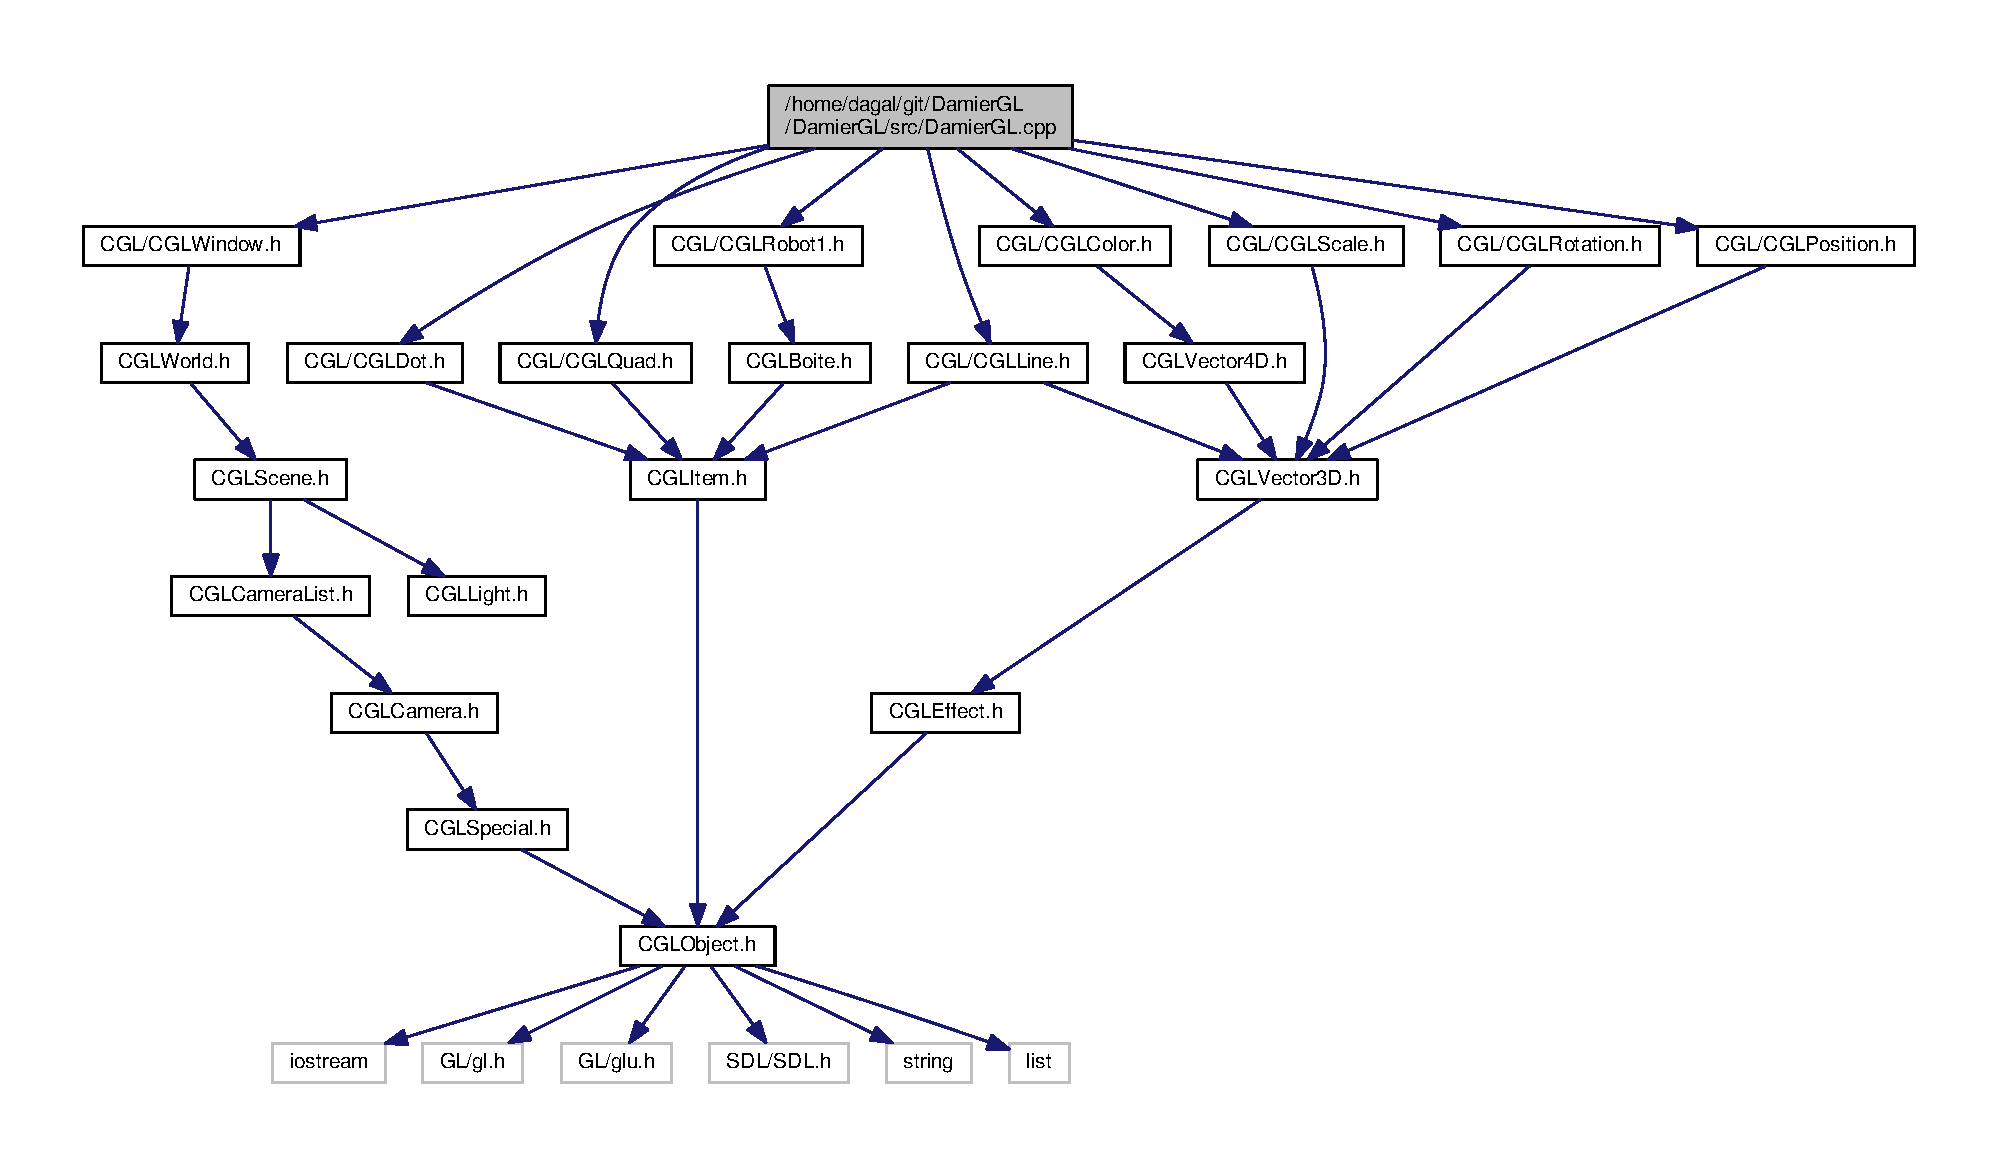
\includegraphics[width=350pt]{d9/dc9/_damier_g_l_8cpp__incl}
\end{center}
\end{figure}
\subsection*{Fonctions}
\begin{DoxyCompactItemize}
\item 
int \hyperlink{_damier_g_l_8cpp_a0ddf1224851353fc92bfbff6f499fa97}{main} (int argc, char $\ast$argv\mbox{[}$\,$\mbox{]})
\end{DoxyCompactItemize}


\subsection{Documentation des fonctions}
\hypertarget{_damier_g_l_8cpp_a0ddf1224851353fc92bfbff6f499fa97}{\index{Damier\-G\-L.\-cpp@{Damier\-G\-L.\-cpp}!main@{main}}
\index{main@{main}!DamierGL.cpp@{Damier\-G\-L.\-cpp}}
\subsubsection[{main}]{\setlength{\rightskip}{0pt plus 5cm}int main (
\begin{DoxyParamCaption}
\item[{int}]{argc, }
\item[{char $\ast$}]{argv\mbox{[}$\,$\mbox{]}}
\end{DoxyParamCaption}
)}}\label{_damier_g_l_8cpp_a0ddf1224851353fc92bfbff6f499fa97}


Définition à la ligne 22 du fichier Damier\-G\-L.\-cpp.



Voici le graphe d'appel pour cette fonction \-:
\nopagebreak
\begin{figure}[H]
\begin{center}
\leavevmode
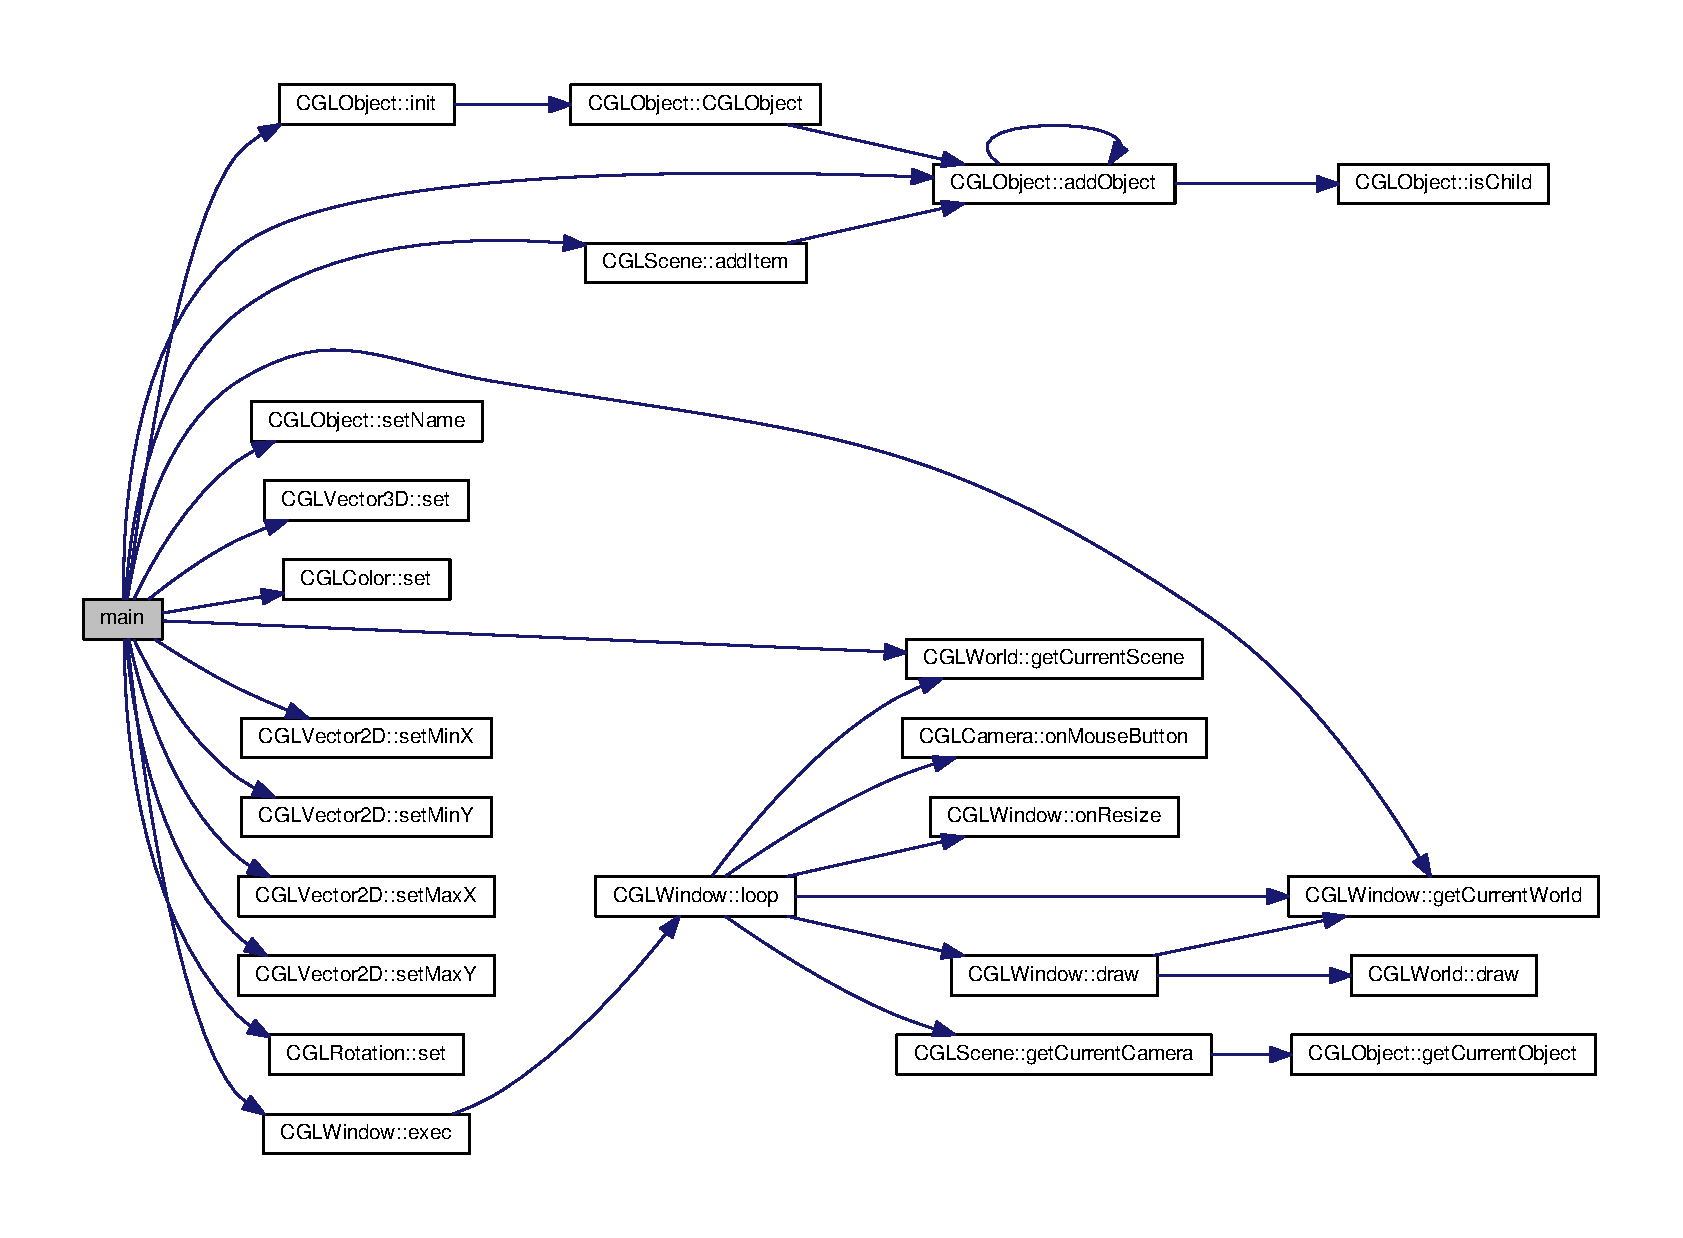
\includegraphics[width=350pt]{db/dec/_damier_g_l_8cpp_a0ddf1224851353fc92bfbff6f499fa97_cgraph}
\end{center}
\end{figure}



%--- End generated contents ---

% Index
\newpage
\phantomsection
\addcontentsline{toc}{chapter}{Index}
\printindex

\end{document}
